\documentclass[12pt]{article}

\usepackage{setspace}
\usepackage{minted}
\usepackage{fancyvrb}
\usepackage{listings}
\usepackage{graphicx}

\usepackage[margin=0.75in]{geometry}
\pagestyle{empty}

\def \name       {Enrique Gavidia}
\def \coursenum  {CSC 415.01}
\def \coursename {Operating Systems Principles}
\def \instructor {Prof. Murphy}
\def \semester   {Spring 2012}
\def \assignment {Homework \# 6}
\def \duedate    {April 27, 2012}

\newcommand {\mytilde} {$\sim$}
\newcommand {\comment}[1] {\textcolor{red}{#1}}
\newcommand {\filename}[1] {\flushleft \textbf{#1}}
\newcommand {\append}[2] {\section*{Appendix #1} \textsl{\large #2}}

\newcommand {\makecover} {
  \begin{titlepage}
    \begin{center}
      \LARGE{\coursenum, \semester \\ \coursename}\\
      \Large{\instructor}\\
      \vfill
      \textbf{\Huge \assignment}\\
      \vfill
      \Large{\name}\\
      \large{\duedate}
    \end{center}
  \end{titlepage}
}

\DefineVerbatimEnvironment {shelloutput} {Verbatim} {fontsize=\scriptsize, numbers=left, frame=lines, commandchars=\%\{\}}

\newcommand {\includesource}[2] {\inputminted[linenos, fontsize=\scriptsize, frame=lines]{#1}{#2}}
\newcommand {\includeoutput}[1] {\VerbatimInput[fontsize=\scriptsize, numbers=left, frame=lines, commandchars=\%\{\}]{#1}}

\begin{document}

\makecover

%---{ Main Content }--------------------------------------------------------------------
\section*{Assignment Description}


%In this assignment, we were tasked with emulating some of the processes of a virtual memory paging mechanism, such as implement a program 
%that would extract the octal representations of page numbers and their offsets from a given virtual address, and implementing
%3 different page-replacement algorithms: \texttt{FIFO}, \texttt{OPT}, and \texttt{LRU}.  Our goal was to compare and analyze the benefits
%of each of these algorithms in terms of the page faults produced for a given number of frames. To visualize it further, we also had to plot
%the output generated by our implementations of the algorithms. Upon doing this, it became clear why the \texttt{OPT} algorithm would be superior
%at managing its resources, were it feasible to implement in a non-controlled setting with an unlimited page reference string.
% 
% 
%This code has been tested to work under \textsl{Windows}, \textsl{Gentoo Linux}, and \textsl{Mac OSX}.
%The implementation for \textsl{Part 1} is under \textbf{Appendix I}, and the \textbf{Part 2} implementation is in \textbf{Appendix III}. 
%The graph of the output comparing the different page replacement algorithms is located under \textbf{Appendix V}.


\section*{Design \& Implementation}


%I implemented my programs in such a way, that I ensured both parts of this assignment were compatible with both the Windows and [Gentoo] Linux operating systems.
%Even though it was only required for the second part of the assignment, I crafted a portable solution for the first part of the assignment as well, as it required
%nothing more than standard C bit-wise operations for masking and shifting to extract the values from the binary memory address.  Additionally, I made it convenient
%to test the extraction of page numbers and offsets with arbitrary values for page sizes, by accepting an optional 2nd command line argument defining the page size
%to use in Kilobytes.
% 
%With the implementation of the page replacement algorithms in \textsl{Part 2}, I tried to refactor the problems into several smaller, more digestible problems, by 
%using a small handful of helper functions. I also took the measure to prevent the randomly generated \texttt{Page Reference String} from containing identical 
%adjacent values, so that the output would be more consistent and closer to the ideal. The graph of the output values demonstrates this, as it bears a reasonably 
%close fit to the estimated downward slopes graphed in the textbook.  I even plugged in the same data sets as the examples in the book to verify the correctness of 
%my algorithms, and got very similar results.


\section*{Improvements}
I would improve it by using linked-lists instead of arrays, to make better use of the system's memorey and allow for larger sets of data.

%Even though certain algorithms like the \texttt{OPT} page replacement strategy are inherently inefficient, I feel I could improve on my particular implementations a 
%bit more to be more efficient, such as re-implementing my stack for the \texttt{LRU} algorithm to consist of pointers rather than indexes. Adding a good visual output
%component for each algorithm would also be a good feature to give the user a bit more understanding about what each algorithm does, and why it arrived at the result it 
%did.


%---{ Appendices }-----------------------------------------------------------------------
\newpage

%----{ Unix }--------------------------------------------------------------------------
\append{I} {Unix Source Code}
\includesource{c}{unix_search.c}

\append{II} {Unix Output}
\filename{Single-core}
\includeoutput{output/unix_search_singlecore.txt}

\filename{Multi-core}
\includeoutput{output/unix_search_multicore.txt}

%----{ Windows }--------------------------------------------------------------------------
\append{III} {Windows Source Code}
%\includesource{c}{win_search.c}

\append{IV} {Windows Output}
\filename{Single-core}
%\includeoutput{output/win_search_singlecore.txt}

\filename{Multi-core}
%\includeoutput{output/win_search_multicore.txt}

%\append{V} {Graph}
% 
% 
%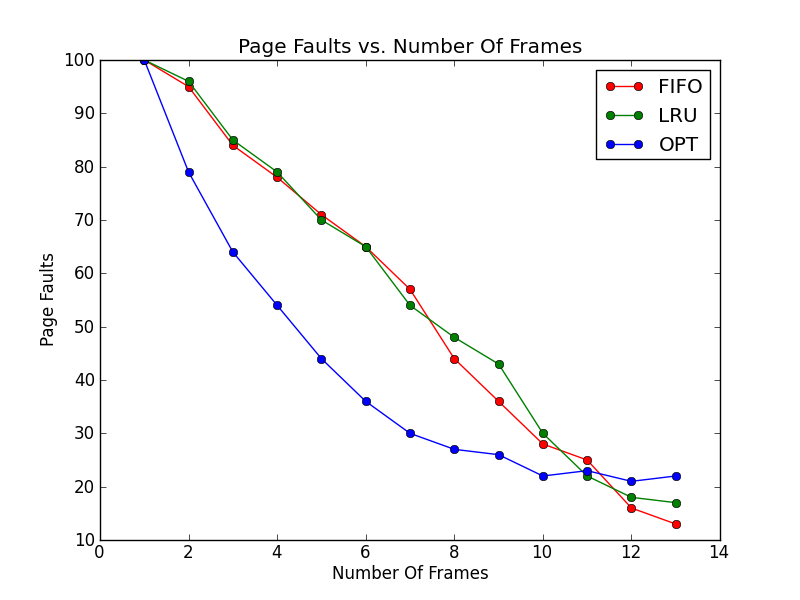
\includegraphics[scale=0.7]{output/graph.png}


\end{document}
